 \chapter{Implementation}\label{C:impl}

\section{Overall Testing Strategy}

As discussed in Section \ref{design}, the overall testing methodology employed in this project was a black-box methodology, and multiple different black-box testing methods were used throughout the course of this project.

\subsection{Testing Environment}

Testing took place on two different systems. The first was a Windows 10 system with an Intel i5-4960k and 8GB of RAM, and the other was an Arch Linux system with an Intel i7-6700k and 16GB of RAM. All tests were run on both systems to make sure any bugs found were due to the compiler code, rather than the environment where the testing was taking place. 

\section{Testing Timeline}

In Section \ref{planTiming}, a planned testing timeline was outlined. It proposed that the initial stages of the project would consist of error guessing testing, as it was thought that it would be the most effective method of testing whilst familiarising with the language. The timeline stated that only a short period of time would be spent using this method before use case testing would be used. 

This was not the case in reality. It took longer than expected to become familiarised with the language, especially in regards to some of the more complicated and unique language features. This meant that usage of error guessing lasted longer than planned (two months compared to one month). The usage of use case testing was not majorly impacted by this, as both testing methods were used in parallel.

Another major difference between the plan and the actual implementation is that the usage of modified orthogonal squares was reduced. It was planned that it would be used in parallel with use case testing for around two months at the end of the project. In reality it was only used for approximately two weeks before it was realised that it provided no real benefit. After a discussion with Dr. Servetto, it was realised that due to the practically infinite input domain, there was little proof it was more effective than purely random testing. After this, use of the modified orthogonal squares testing was discontinued.

This meant that majority of testing that took place over the course of this project was use case testing.

\begin{figure}[h]
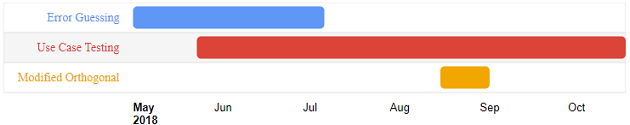
\includegraphics{nis}
\caption{The actual time period of each testing method}
\end{figure}

\section{Techniques Used \label{testMethods}}

\subsection{Error Guessing}

Error guessing, as described in Section \ref{bbtest}, was used over the course of this project. Error guessing was mainly employed at the start of the project as it was a useful testing technique while still familiarising with the language. Error guessing allows the user to take advantage of their previous testing experience. This fact proved useful within this project as research had been done into common compiler bugs. 

Over the course of the project, error guessing found four bugs. The bugs found with error guessing were all bugs in the 42 standard library - Adam's Towel. 

A test developed with error guessing would generally start with a scenario being considered. These scenarios would generally relate to common programming language bugs such as division by zero or invalid method parameters. A program would then be created that used this scenario in some way. This program would then be compiled and run and the result would checked and compared against the expected outcome.

While error guessing and use case testing both used an initial scenario to create the test there were major differences between the two methods. A scenario would be significantly more formal in use case testing as opposed to error guessing. The scenario would also be a lot more carefully followed in use case testing, rather than error guessing.

An example of a test created with error guessing can be seen in Figure \ref{errorguess}. This test was created when the issue of division by zero was considered. A program was written to check what happens when a number is divided by zero. It was decided that the expected outcome of division by zero would be some kind of math error. When the program was created and run, the actual result of one divided by zero was the fraction $\frac{1}{0}$. This test clearly found an error as the actual result ($\frac{1}{0}$) differed from the expected result (an error).

\begin{figure}[h]
	\begin{42listing}
	A: {
		class method divide(Num a, Num b) (
			return a / b
		)
	}
	
	B: {
		Num n = A.divide(a: 1Num, b: 0Num) // We would expect this method call to throw an error.
	}
	\end{42listing}
	\caption{An example of a 42 program created with the error guessing technique \label{errorguess}}
\end{figure}

Another example of a test created with error guessing would include passing different types of parameters to standard library methods than the methods expect. Overall an error guessing test would generally involve writing a 42 program that was not quite syntactically or type correct, and comparing the actual output of the program against what would be expected.



\subsection{Use Case Testing}

Use case testing as described in Section \ref{bbtest} was used in this project. Use case testing was employed throughout the majority of the time of this project and it proved to be extremely useful and effective. One thing to note about the use case testing that was employed in this project was that, compared to the more usual usage of this testing method, the use cases are lower level and focus more on the specific actions that a programmer wants their program to do. The use cases are not fully system orientated, they are still partially user orientated, like use case testing calls for.

A test developed with use case testing would generally follow a set structure. Firstly, a list of actions that would be carried out by a program would be created. The program would then be created using the list of actions as guidelines. This program would then have the actual output compared against the expected output. If the outputs differed, or if an error was thrown, a bug had been identified.

This method of testing allowed for a broad range of programs, and therefore tests, to be created. This is because a use case could be created to target any specific part of the language. For example it is easy to create a use case that tests lists, or a use case that tests inheritance. This allowed for use case testing to test parts of the language that were not covered by other methods of testing. Additionally it allowed for testing of parts of the language that were considered to be more likely to have bugs but would have been difficult to test with other methods. Examples of this include inheritance, which would have been difficult to test with other methods, but was fairly simple with use case testing. 

A scenario of a Cat and Dog class implementing an Animal interface was created. A program was then created, compiled, and run from this scenario. It was then decided to test what would happen if the Dog class was to implement an additional interface. To facilitate this, the scenario and test were simply updated. This was a simple process, and it illustrates the flexibility that use case testing brought to this project.

\begin{figure}[ht]
	\centering
\textbf{Scenario for finding the maximum value in a list of numbers}
	\begin{enumerate}
		\item{Create a list of numbers.}
		\item{Check if the list of numbers is empty.}
		\item{Create a variable that will hold the current maximum value at any point in time.}
		\item{Iterate through the list and check if each number in the list is larger than current maximum. If so, update the current maximum.}
		\item{Return the current maximum value.}
		\item{Assert method result is equal to max list value.}
	\end{enumerate}
	\caption{A list of actions for a program that finds the minimum value in a list of numbers \label{actions}}
	~\\
	\end{figure}

\begin{figure}[ht]
		\begin{42listing}
		A: {
			class method Num max(Nums list) {
				if list.isEmpty() ( // Step 2
					error Undefined"Empty list!"
				)
				
				var Num max = list.val(0Size) // Step 3
				with e in list.vals() ( // Step 4
					if e > max (
						max := e
					)
				)
				return max // Step 5
			}
			
			Nums list = Nums[1Num; 55Num; 0Num; 12Num; 32Num] // Step 1
			X[max(list: list) == 55Num] // Step 6
		}
		\end{42listing}
		\caption{The code for a 42 program that meets the list of actions in \ref{actions}. It is an example of a test created with use case testing \label{figMax}}
\end{figure}

An example of use case testing could be to find the maximum value of a list of numbers and it is shown in Figures \ref{actions} and \ref{figMax}.



\subsection{Orthogonal Squares}

The modified orthogonal squares method (as described in Section \ref{bbtest}) was used during this project. Unfortunately it did not prove to be very effective over the course of this project. It was realised that it did not provide any real benefit over either use case testing or error guessing. After around a week using the method for testing it was realised that it was not producing the desired result (of finding bugs). This led to discussion with Dr. Servetto where it was decided that the method may not have been suitable for testing during this project. It was realised that the 42 compiler is very difficult to test with this method, due to the language itself (e.g. arbitrary-precision numbers, no character class). Additionally Dr. Servetto pointed out that there was no proof the method was any more beneficial than a purely random approach. Due to this it was decided that any testing with this method would be ceased and instead replaced with more use case testing, as it had already proven to be successful. 

The decision to stop using this testing method was backed up by the fact that while it was in use, not a single bug was found with it.



\section{Developed Tools}

\subsection{42TestHelper \label{42TestHelper}}


When a program was written and it was considered to be "interesting" enough to turn it into a test, it would be converted from 42 code to a JUnit \cite{junit} test that would run in the 42 automated test suite, which is written in Java.

\begin{figure}[h]

	\begin{42listing}
	Nums: Collections.vector(of: Num)
	A: {
		primes = Nums[2Num; 11Num; 13Num; 17Num; 19Num]
		var Num initial = 2520Num
		with prime in primes.vals() (
			initial := initial * prime
		)
		return ExitCode.normal()
	}
	\end{42listing}
	\caption{An example of a 42 program \label{42code} that could be turned into a JUnit test}
\end{figure}

\begin{figure}[h]		

\begin{lstlisting}
	@Test
	public void testPrimes() {
		tp("{reuse L42.is/AdamTowel02"
			,"Nums: Collections.vector(of: Num)"
				,"A: {"
			    	,"primes = Nums[2Num; 11Num; 13Num; 17Num; 19Num]"
			    	,"var Num initial = 2520Num"
					,"with prime in primes.vals("
						,"(initial := initial * prime)"
					,")"
			    	,"return ExitCode.normal()"
				,"}"
		,"}");
	}		

\end{lstlisting} 
\caption{The 42 program from Figure \ref{42code} turned into a JUnit test \label{javacode}}
\end{figure}

As seen in Figure \ref{javacode}, turning a 42 program into a test for the 42 test suite requires the creation of a JUnit test that calls a method \textit{tp} that takes a variable number of arguments. Each argument is a string that represents a line of the 42 program. When a test is constructed, the standard JUnit boilerplate is created before the 42 program is turned into a series of strings that are passed as arguments to the \textit{tp} method. This is a fairly time consuming process when done manually, especially when many tests are created at once, or a 42 program is long. During the initial stages of the project, the conversion of 42 programs to JUnit tests was done manually by hand. It was then realised that this could be easily automated as the process required little thinking. A Python tool was created \cite{pytest} that turned 42 code in a JUnit test and could also turn a JUnit test, assuming it contained valid 42 code, into 42 code. A web version of the tool was also created \cite{jstest}. 


This tool greatly sped up the conversion of 42 programs to tests, and allowed the rapid creation of tests, saving significant amounts of time. 

\section{Test Creation Process}

The process of turning a 42 program that had been created with one of the testing methods discussed in Section \ref{testMethods} was fairly straightforward. A program would be created with an expected output, and then the program would be compiled and run. The actual output of the program would then be compared to the expected output.

 If the outputs matched, and no unexpected error was thrown, no bug had been found. In this case, a decision was then made if the program would make an "interesting" test. The "interestingness" of a test was based on how similar the program was to other tests, if it used any unusual language features or syntax, and the result. If a test was deemed to be "interesting" it would then be converted to a JUnit test through the use of the 42TestHelper (see Section \ref{42TestHelper}) and added to the 42 automated test suite.

If the actual and expected output did not match, it was considered likely that a bug had been found. The code would then be minimised, by removing the code which was not necessary to trigger the bug, and it would be checked if the bug had already been found and reported. If not, the bug would be converted into a JUnit test with the 42TestHelper (see Section \ref{42TestHelper}). It would then be added to the 42 automated test suite.

\begin{figure}[h]
\centering
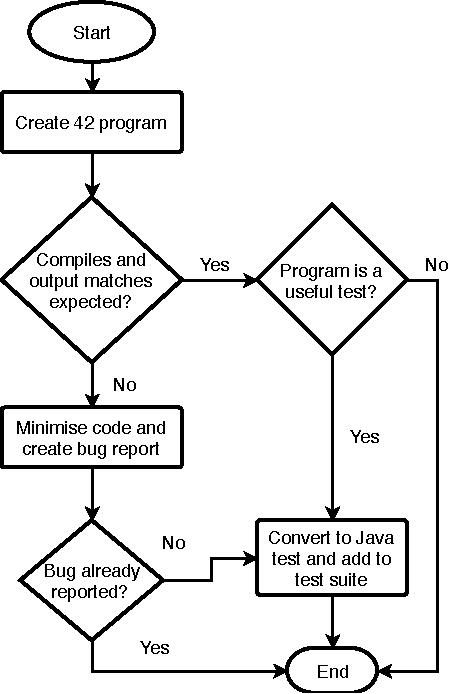
\includegraphics{flowchart}
\caption{A flowchart of creating a standard 42 test}
\end{figure}
